\newpage
%%%%%%%%%%%%%%%%%%%%%%%%%%%%%%%%%%%%%%%%%%%%%%%%%%%%%%%%%%%%%%%%%%%%%%%%%%%%%%%%%%%%%%%%%%%%%%%%%%%%%%%%%%%%%%%%%%%%%
\section{Objetivo}
El objetivo del presente proyecto es definir y justificar los datos y características constructivas y técnicas necesarios para la realización de la instalación eléctrica automatización de una fábrica de complementos alimenticios, exponiendo ante los organismos competentes que la instalación que nos ocupa reúne las condiciones y garantías exigidas por la reglamentación vigente, a fin de obtener la Autorización Administrativa y la de Ejecución de la instalación por parte de la Dirección General de Industria, Energía y Minas, Gobierno de la Comunidad de Madrid y Ayuntamiento de Rivas-Vaciamadrid.\
 
%%%%%%%%%%%%%%%%%%%%%%%%%%%%%%%%%%%%%%%%%%%%%%%%%%%%%%%%%%%%%%%%%%%%%%%%%%%%%%%%%%%%%%%%%%%%%%%%%%%%%%%%%%%%%%%%%%%%%
\section{Ubicacion}

La Instalación objeto del presente proyecto se realizará en una nave industrial construida en el año 1992 ubicada en la siguiente dirección:\\

 {\bfseries Calle de la Fundición 8, Rivas-Vaciamadrid, Comunidad de Madrid, (España)}

%%%%%%%%%%%%%%%%%%%%%%%%%%%%%%%%%%%%%%%%%%%%%%%%%%%%%%%%%%%%%%%%%%%%%%%%%%%%%%%%%%%%%%%%%%%%%%%%%%%%%%%%%%%%%%%%%%%%%
\section{Antecedentes}

La nave industrial en la cual se realizará la instalación objeto de este proyecto estuvo ocupada por un concesionario y taller de reparación de automóviles desde el año 1992 hasta el año 2013. La propiedad adquirió la nave industrial en el año 2013 con el objetivo de reconvertir el espacio en una fábrica de complementos alimenticios, dada la fuerte demanda que está teniendo este tipo de productos en los últimos años. Las instalaciones eléctricas de se desmantelaron para la reconversión, siendo su diseño parte del objeto de este proyecto.\

%%%%%%%%%%%%%%%%%%%%%%%%%%%%%%%%%%%%%%%%%%%%%%%%%%%%%%%%%%%%%%%%%%%%%%%%%%%%%%%%%%%%%%%%%%%%%%%%%%%%%%%%%%%%%%%%%%%%%
\section{Normativa}

En el estudio y redacción del siguiente proyecto se han tenido en cuenta las siguientes normas y reglamentos actualmente en vigor:\\

{\bfseries Ley 54/1997 de 27 de Noviembre, de Regulación del Sector Eléctrico} (B.O.E. 28 de Noviembre de 1997).\\

{\bfseries Real Decreto 1995/2000}, de 1 de diciembre, por el que se regulan las actividades de transporte, distribución, comercialización, suministro y procedimientos de autorización de instalaciones de energía eléctrica.\\

{\bfseries Reglamento Electrotécnico para Baja Tensión. (R.E.B.T.)}\
Real Decreto 842/2002 de 2 de agosto.\\

{\bfseries Orden de 13-03-2002 de la Consejería de Industria y Trabajo}, por la que se establece el contenido mínimo en proyectos de industrias y de instalaciones Industriales.\\

{\bfseries Código Técnico de la Edificación.} (C.T.E.) Real Decreto 314/2006, de 17 de marzo.\\

{\bfseries Normas UNE, UNE-EN, EN e IEC}\\

{\bfseries Normas particulares de la Compañía Suministradora.}\\

{\bfseries Ordenanzas Municipales del Ayuntamiento de Rivas-Vaciamadrid.}\\

{\bfseries Directiva 2002/46/CE} del Parlamento Europeo y del Consejo, de 10 de junio de 2002, relativa a la aproximación de las legislaciones de los Estados miembros en materia de complementos alimenticios.\\

{\bfseries Reglamento (CE) 1137/2008} del Parlamento Europeo y del Consejo, de 22 de octubre de 2008 , por el que se adaptan a la Decisión 1999/468/CE del Consejo determinados actos sujetos al procedimiento establecido en el artículo 251 del Tratado, en lo que se refiere al procedimiento de reglamentación con control.\\

{\bfseries Reglamento (CE) n o 1170/2009} de la Comisión, de 30 de noviembre de 2009 , por la que se modifican la Directiva 2002/46/CE del Parlamento Europeo y del Consejo y el Reglamento (CE) n o 1925/2006 del Parlamento Europeo y del Consejo en lo relativo a las listas de vitaminas y minerales y sus formas que pueden añadirse a los alimentos, incluidos los complementos alimenticios.\\

{\bfseries Real Decreto 1487/2009}, de 26 de septiembre, relativo a los complementos
alimenticios.\\

{\bfseries Otros reglamentos vigentes que le sean de aplicación.}\\

En caso de producirse alguna diferencia de criterio entre una normativa y otra debe permanecer la de rango superior, siempre y cuando la de rango inferior no fuese más perceptiva.

%%%%%%%%%%%%%%%%%%%%%%%%%%%%%%%%%%%%%%%%%%%%%%%%%%%%%%%%%%%%%%%%%%%%%%%%%%%%%%%%%%%%%%%%%%%%%%%%%%%%%%%%%%%%%%%%%%%%%
\section{Descripción general}

DESCRIPCION DEL PROYECTO\\
 
El edificio se compone de dos áreas diferenciadas: una zona de oficinas de dos plantas con una superficie útil por planta de 175$m^2$ y la zona industrial con una superficie útil de 1260$m^2$, siendo la {\bfseries superficie total 1610\mbox{\boldmath${m^2}$}}\\



El recinto tiene una superficie de ??????????? metros cuadrados, incluyendo la nave con las oficinas y un espacio de maniobra para camiones.
La nave tiene una superficie útil de ????????? metros cuadrados y se divide en tres zonas distintas: zona de carga y descarga de materiales, zona de almacenamiento de materia prima, zona de almacenamiento del produto finalizado y zona de máquinas donde se realiza el proceso de fabricación.
\\

Los camiones entran por en el recinto y tras maniobrar en el espacio habilitado para ello entran marcha atrás en la nave, donde los empleados procederán a descargarlo con la ayuda de toros mecánicos. Los sacos con la materia prima en polvo, así como los cartones para ensamblar las cajas, se almacenan en estanterías de palés situados delante del inicio del proceso. 
\\

En la zona de máquinas se lleva a cabo todo el proceso de transformación del polvo a cajas de pastillas. Contiene un horno de polvo, una máquina de compresión, una máquina de pruebas, un tambor de revestimiento, una máquina de formación de blisters y una última de embalaje, así como cintas para transportar los distintos elementos y dos brazos robóticos para colocar el producto final. El producto final se almacena en palés en estanterías cerca de la puerta para agilizar el proceso de carga del camión y por tanto perder menos tiempo.
\\

El espacio de oficinas cosiste de una recepción y un centro de control en la planta baja y un despacho y puestos de trabajo en el segundo nivel. Ambos pisos disponen de baños.





%%%%%%%%%%%%%%%%%%%%%%%%%%%%%%%%%%%%%%%%%%%%%%%%%%%%%%%%%%%%%%%%%%%%%%%%%%%%%%%%%%%%%%%%%%%%%%%%%%%%%%%%%%%%%%%%%%%%% 
\section{Elementos del sistema}

\subsection{Instalación eléctrica}

\subsubsection{Red de suministro}

La empresa encargada de suministrar energía eléctrica a la instalación será UNIÓN FENOSA, S.A.\\

Características de la red de suministro:\

\begin{itemize}
\item {\bfseries Red:} Corriente Alterna Trifásica 
\item {\bfseries Tensión:} 400/230 V (Entre fases y entre fase y neutro)
\item {\bfseries Frecuencia:} 50 Hz
\item {\bfseries Intensidad de cortocircuito trifásico:} 12 kA
\end{itemize}

El suministro se realizará a través de {\bfseries Acometida Subterránea con conductores unipolares de aluminio RV 0,6/1 kV 3 x 240 + 1 x 150 Al} instalados bajo tubo enterrado, llegando a una CGP de instalación empotrada. La instalación será existente, siendo sólo objeto de este proyecto la instalación aguas abajo a partir del Cuadro General de Mando y Protección cuya envolvente se ajusta a las normas UNE 20.451 y UNE-EN 60.439 -3, con un grado de protección IP 30 según UNE 20.324 e IK07 según UNE-EN 50.102.\\

Para la sección de conductores indicada previamente, teniendo en cuenta sus características de instalación y que los fusibles instalados en la CGP son de (( 160A o 200A, se prevé una potencia máxima admisible en la instalación de:XXXXXXkW



\subsubsection{Previsión de potencia}

La nave industrial contará con las siguientes cargas y receptores:\\

\begin{itemize}
\item Tomas de corriente 2.300 W
\item Alumbrado Incandescente xx luminarias de 30 W 
\item Alumbrado fluorescente xx luminarias de 4x36 W 
\end{itemize}

La potencia total prevista para el edificio será de XXXXX W.

El resto de información y cálculos se encuentran en el {\bfseries Anexo Nº X(Cálculos Justificativos)} del presente proyecto.

\subsubsection{Cuadro General de Mando y Protección}

ORGANIZAR

Tres cuadros bla bla

Los dispositivos generales e individuales de mando y protección serán, como mínimo:

Interruptor general automático de corte omnipolar, que permita su accionamiento manual y que esté dotado de elementos de protección contra sobrecarga y cortocircuitos. Este interruptor será independiente del interruptor de control de potencia.\\



La sensibilidad de los interruptores diferenciales responderá a lo señalado en la Instrucción ITC-BT-24.
Todas los Interruptores Automáticos Magnetotérmicos (IAM) serán de corte omnipolar, tipo de curva C y poseerán un poder de corte de 6 kA. (Schneider Electric Gama Domae)

Se seleccionarán protecciones con un poder de corte de 6 kA al ser más económicos que los de poder de corte 4,5 kA que se exigen como mínimo por normativa.

Los interruptores diferenciales serán de la marca Schneider Electric Gama Domae.

Las especificaciones particulares de cada cuadro, servicios generales o local comercial se encuentran detalladas en el ANEXO TAL

\subsubsection{Instalación eléctrica de la oficina}

libres de alógenos

Es la parte de la instalación eléctrica que partiendo del Cuadro de Mando y Protección de la Oficina, enlaza con los receptores de iluminación, tomas de corriente de uso general, tomas de corriente de baño y tomas de corriente SAI.\\

Está regulada en las ITC-BT 25 e ITC-BT 26 del R.E.B.T. donde se especifican las prescripciones generales de instalación y calibres de los tubos a utilizar en cada circuito. Los conductores utilizados para estos circuitos serán de cobre unipolares con aislamiento de cobre y una tensión asignada de 450/750 V (H07V-K). La instalación de estos conductores realizará bajo tubo curvable de 2 capas en montaje empotrado en pared de mampostería.

\subsubsection{Instalación elécrtica de la zona de fabricación y almacén}






La caída de tensión sera como máximo del 5\%. Esta caída de tensión se calculará para una intensidad de funcionamiento del circuito igual a la intensidad nominal del interruptor automático de dicho circuito y para una distancia correspondiente a la del punto de utilización mas alejado del origen de la instalación. El valor de la caída de tensión podrá compensarse entre el de la instalación eléctrica de la oficina y el de la derivación del Cuadro General de Mando y Protección (CGMP) al Cuadro de Mando y Protección de la Oficina, de forma que la caída de tensión total sea inferior a la suma de los valores límite especificados para ambas.\\

Los conductores de la instalación deben ser fácilmente identificados, especialmente por lo que respecta a los conductores neutro y de protección. Esta identificación se realizará por los colores que presenten sus aislamientos. Cuando exista conductor neutro en la instalación o se prevea para un conductor de fase su pase posterior a conductor neutro, se identificarán éstos por el color azul claro. Al conductor de protección se le identificará por el doble color amarillo-verde. Todos los conductores de fase, o en su caso, aquellos para los que no se prevea su pase posterior a neutro, se identificarán por los colores marrón o negro. Solamente cuando se considere necesario identificar tres fases diferentes, podrá utilizarse el color gris.\\

En la ejecución de las instalaciones interiores de las viviendas se deberá tener en cuenta:
No se utilizará un mismo conductor neutro para varios circuitos. Todo conductor debe poder seccionarse en cualquier punto de la instalación en el que se realice una derivación del mismo, utilizando un dispositivo apropiado, tal como un borne de conexión, de forma que permita la separación completa de cada parte del circuito del resto de la instalación.\\

En ningún caso se permitirá la unión de conductores mediante conexiones y o derivaciones por simple retorcimiento o arrollamiento entre sí de los conductores, sino que deberá realizarse siempre utilizando bornes de conexión montados individualmente o constituyendo bloques o regletas de conexión. Siempre deberán realizarse en el interior de cajas de empalme y / o derivación (Según ITC-BT 19).\\

Los materiales seleccionados para el presente proyecto son los siguientes:

-	Tomas de Corriente C2A (Schuko): BJC Serie Iris (Blanco) o equivalente.
-	Mecanismos (Interruptores, Conmutadores, Conmutadores de Cruce, Tomas de TV y TP): BJC Serie Iris sin difusor (Blanco) o equivalente.
-	Iluminación incandescente: Lámparas halógenas Phillips Fugato Micro (Orientable) o equivalente.
-	Iluminación fluorescente: Luminarias fluorescentes Phillips M2-BD45 o equivalentes.
En el local comercial se realizará una instalación provisional de iluminación y tomas de corriente de uso general al conformar en si mismo un proyecto independiente no objeto del presente proyecto.

Las Intensidades Máximas Admisibles de los conductores se regirán en su totalidad por lo indicado en la norma UNE 20460-5-523.

Las secciones de los conductores utilizados para los diferentes circuitos, así como el diámetro exterior de los tubos instalados, aparecen reflejados en el Anexo Nº I (Cálculos Justificativos) del presente proyecto, así como en los esquemas adjuntos.



\subsection{Maquinaria}
	\subsubsection{Máquina de secado de polvo}
	\subsubsection{Máquina de compresión en tabletas}
	\subsubsection{Máquina de verificación de dureza de tabletas}
	\subsubsection{Máquina de revestimiento de tabletas}
	\subsubsection{Máquina de sellado de blisters }
	
	\subsubsection{Máquina de empaquetado}
	\subsubsection{Robot de paletizado}
%%%%%%%%%%%%%%%%%%%%%%%%%%%%%%%%%%%%%%%%%%%%%%%%%%%%%%%%%%%%%%%%%%%%%%%%%%%%%%%%%%%%%%%%%%%%%%%%%%%%%%%%%%%%%%%%%%%%%	
\section{Sistema propuesto}


Cuando el horno emita una señal de aviso un operario procederá a llenar el depósito de dicho horno con la materia prima. Una vez lleno, el horno libera el polvo uniformemente sobre una cinta transportadora. Esta lo transporta por el horno de manera ondulante para eliminar cualquier tipo de humedad. 
\\

A la salida del horno el polvo es introducido en una máquina de compresión, donde es convertido en pastillas y se le imprime el nombre de la pastilla.  Acto seguido pasa por una máquina de comprobación, que desecha cualquier pastilla que haya resultado demasiado frágil por seguir húmeda tras el horno. Las pastillas desechadas, se trituran y depositan en un recipiente para que el operario lo reintroduzca en el horno en la siguiente iteración. 
\\

El resto de pastillas continúa hasta un tambor donde se les da un revestimiento de agua con colorantes para su identificación y conservación, al endurecer así la capa exterior y evitar que se deshagan. Tras ser rociadas por pulsos muy rápidos y cortos para favorecer un secado rápido son transportadas a una máquina de sellado.
\\

En esta máquina se dejan caer pastillas hasta llenar un depósito, donde mediante un sensor indica el llenado. La selladora coloca las pastillas en posición segun la matriz utilizada. Paralelamente tira del rollo de plástico en lámina y lo coloca debajo de la parte superior. Al bajar, ésta deforma la lámina con unos cabezales calientes y crea los habitáculos donde inmediatamente inserta las tabletas. Acto seguido se corta el plástico y este avanza a la siguiente posición donde se le coloca una lámina de alumnio con el logo impreso y es sellado por calor al bajar la parte superior en la siguiente iteración. 
\\

Finalmente se transportan los blisters sellados por otra cinta transportadora a la máquina de empaquetado, que coge las cartulinas de las cajas y las dobla para darles su forma final e inserta los blisters en la caja, asi como un folleto explicativo previamente impreso y doblado. Las cajas con el produto final se dejan caer por una rampa hasta una mesa donde un brazo robótico equipado con una cámara coge las cajas individuales y las coloca en cajas de lotes en un palé para ser recogido por un operario y almacenado en una estantería. Un segundo brazo robótico coje un palé de una pila de palés vacíos y lo coloca en la posición del anterior.
\\
%%%%%%%%%%%%%%%%%%%%%%%%%%%%%%%%%%%%%%%%%%%%%%%%%%%%%%%%%%%%%%%%%%%%%%%%%%%%%%%%%%%%%%%%%%%%%%%%%%%%%%%%%%%%%%%%%%%%%
\section{Flujograma}
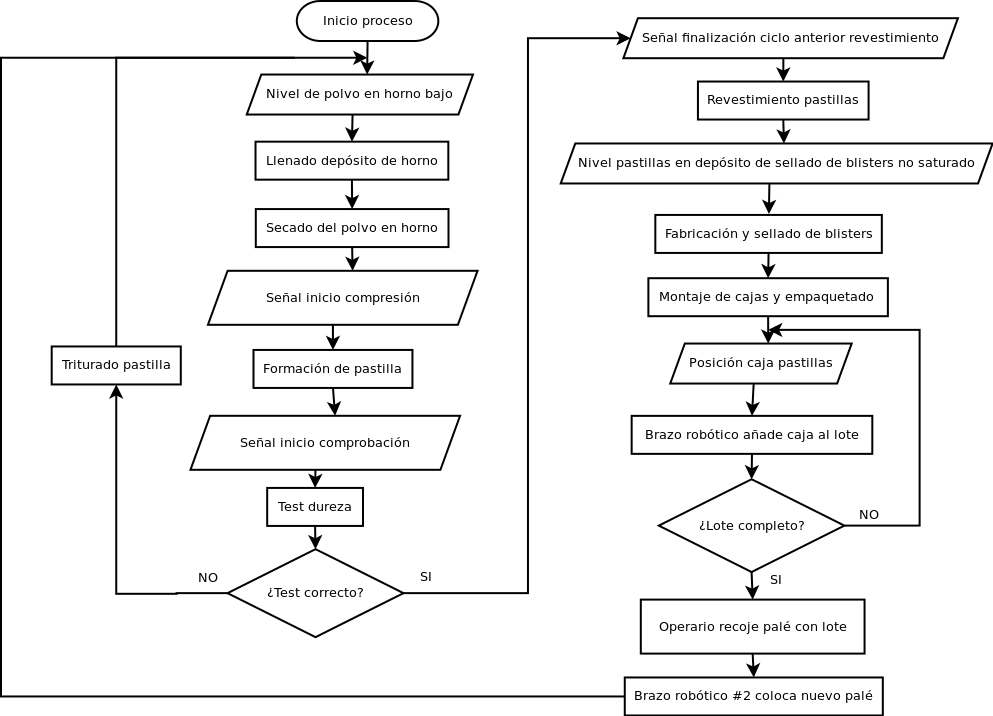
\includegraphics[width=15cm,height=20cm,keepaspectratio]{Planos/Flujograma.png}



%%%%%%%%%%%%%%%%%%%%%%%%%%%%%%%%%%%%%%%%%%%%%%%%%%%%%%%%%%%%%%%%%%%%%%%%%%%%%%%%%%%%%%%%%%%%%%%%%%%%%%%%%%%%%%%%%%%%%%%%%%%%%%%%
\newpage\section {Firmas de los ingenieros}
\vspace{5cm}
Fdo. Alvaro Ferrán Cifuentes
\vspace{5cm}\hspace{5cm}
Fdo. David Antón Sánchez

%%%%%%%%%%%%%%%%%%%%%%%%%%%%%%%%%%%%%%%%%%%%%%%%%%%%%%%%%%%%%%%%%%%%%%%%%%%%%%%%%%%%%%%%%%%%%%%%%%%%%%%%%%%%%%%%%%%%%
\newpage \section{Anexos}

   
\subsection{Anexo de cálculos:}

\subsubsection{Cálculos de la Instalación eléctrica}
\paragraph{Diseño del cuadro general de protección y mando}
\paragraph{Cálculo de las líneas de alimentación de cada máquina}
\paragraph{Cálculo de las líneas para las tomas de corriente de uso general}
\paragraph{Cálculo de las líneas para las tomas de corriente con SAI}
\paragraph{Cálculo de las líneas para iluminación}
\paragraph{Cálculo de las líneas para iluminación de emergencia}

\subsubsection{Cálculo de las instalaciones de automatización}
\paragraph{Sensores }
\paragraph{Cuadro centralización de automatización}
\paragraph{Rack con PC industrial conectado a la red de la fábrica}
\subsubsection{Instalaciones de seguridad}
\paragraph{Protección de las personas}
\paragraph{Protección contra intrusión}

\subsection{Anexo de código}
\newpage
\subsection{Anexo de catálogos}
\subsubsection{Máquina de secado de polvo}
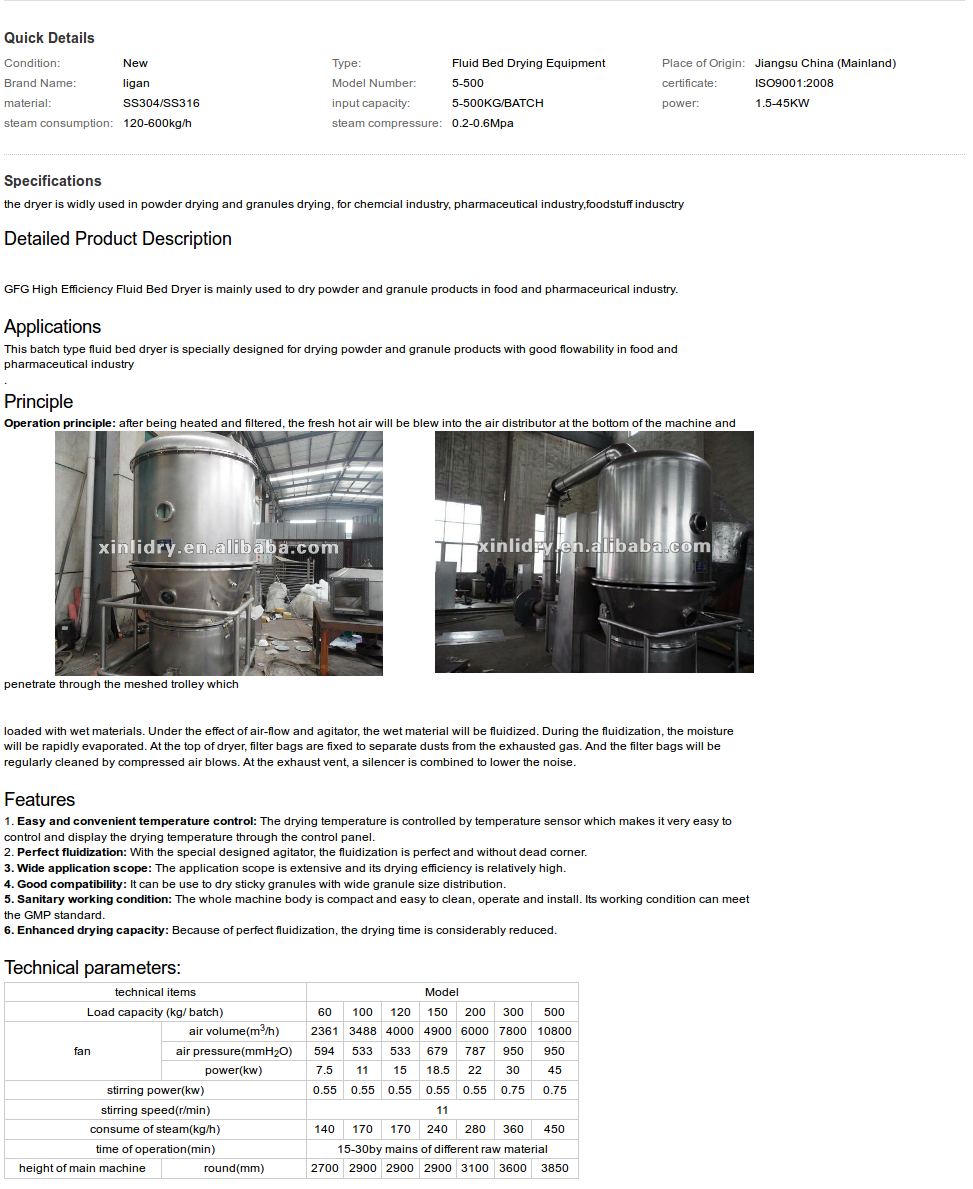
\includegraphics[width=15cm,height=20cm,keepaspectratio]{Datasheets/1MaquinaSecado.png} 
\newpage

\subsubsection{Máquina de compresión en tabletas}

\includegraphics[width=15cm,height=20cm,keepaspectratio]{Datasheets/2MaquinaPrensado.png} 
\newpage

\subsubsection{Máquina de verificación de dureza de tabletas}
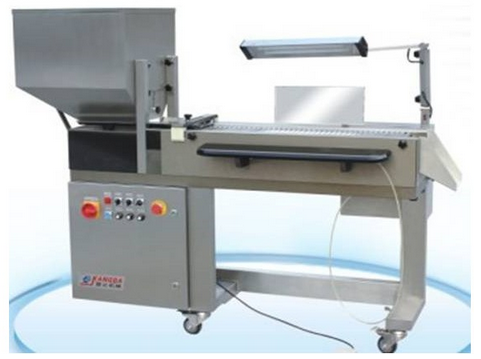
\includegraphics[width=5cm,height=4cm,keepaspectratio]{Datasheets/3Foto.png} 
\\

\includegraphics[width=15cm,height=20cm,keepaspectratio]{Datasheets/3MaquinaVerificacion.png} 
\newpage

\subsubsection{Máquina de revestimento de tabletas}
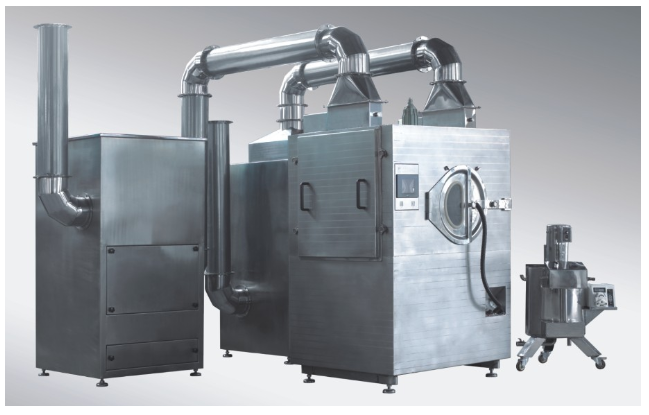
\includegraphics[width=5cm,height=4cm,keepaspectratio]{Datasheets/4Foto.png} 
\\
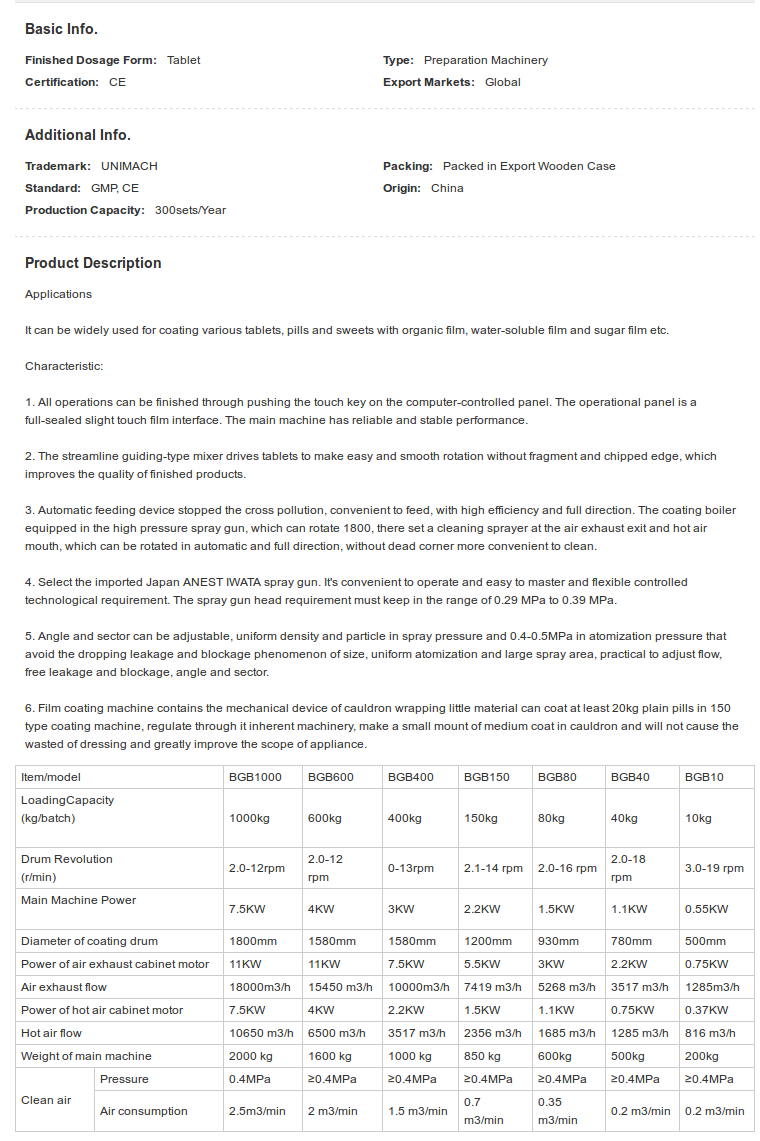
\includegraphics[width=15cm,height=20cm,keepaspectratio]{Datasheets/4MaquinaRevestimiento.png} 
\newpage

\subsubsection{Máquina de sellado de blisters}
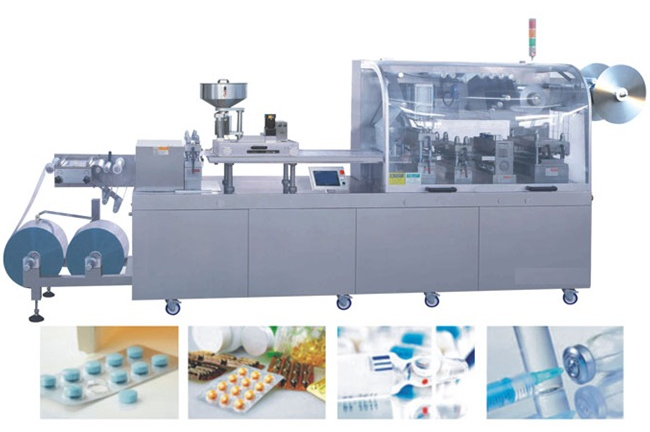
\includegraphics[width=5cm,height=4cm,keepaspectratio]{Datasheets/5Foto.png} 
\\

\includegraphics[width=15cm,height=20cm,keepaspectratio]{Datasheets/5MaquinaBlisters.png} 
\newpage

\subsubsection{Máquina de empaquetado}
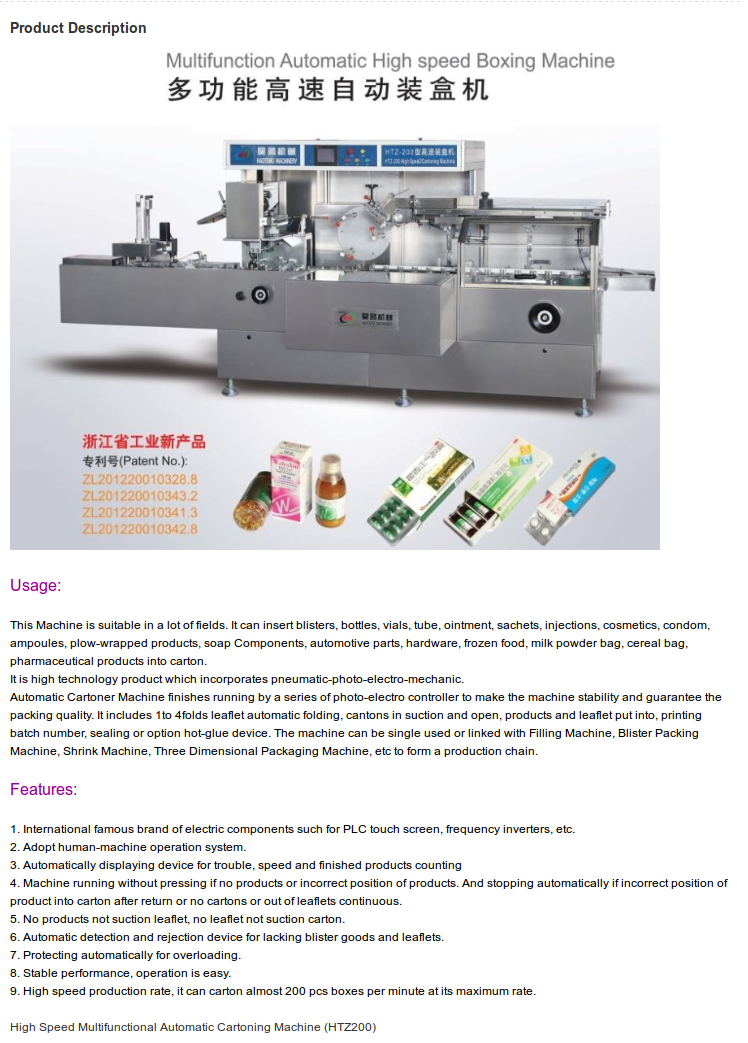
\includegraphics[width=15cm,height=20cm,keepaspectratio]{Datasheets/7MaquinaEmpaquetado.png} 
\newpage
\subsubsection{Robot de paletizado}

\subsection{Planificación}

